% Adding a coloured vertical edge to the pages in the chapter
\ClearShipoutPicture
\AddToShipoutPicture{%
  \AtPageLowerLeft{%
    \checkoddpage
    \ifoddpage
      \begin{tikzpicture}[remember picture,overlay] % Odd page → right edge
        \draw[line width=80pt, colour_chapter7] 
             (\paperwidth,0) -- (\paperwidth,\paperheight);
      \end{tikzpicture}%
    \else
      \begin{tikzpicture}[remember picture,overlay] % Even page → left edge
        \draw[line width=80pt, colour_chapter7] 
             (0,0) -- (0,\paperheight);
      \end{tikzpicture}%
    \fi
  }%
}

%%%%%%%%%%%%%%%%%%%%%%%%%%%%%%%%%%%%%%%%%%%%%%%%%%%%%%%%%%%%%
\chapter{Towards predictions over a continuous global domain: 
global implementation of regionally-trained models}
\label{regional_to_global_training}
\graphicspath{{chapter_07/figures}{chapter_07/tables}}
%%%%%%%%%%%%%%%%%%%%%%%%%%%%%%%%%%%%%%%%%%%%%%%%%%%%%%%%%%%%%

\underline{\textbf{Authors' contribution for this chapter:}} Fatima M. Pillosu designed the study, with advice from Hannah Cloke and Christel Prudhomme, obtained the datasets, carried out the analysis, and led the writing of the manuscript. All authors assisted with writing the manuscript. Overall, 90\% of the writing was undertaken by Fatima M. Pillosu.

\vspace{\baselineskip}

\section*{PREFACE}
\addcontentsline{toc}{section}{PREFACE}



\clearpage

\section*{ABSTRACT}
\addcontentsline{toc}{section}{ABSTRACT}

\clearpage



%%%%%%%%%%%%%%%%%%%%%%
\section{Introduction}

The aspiration to develop predictions of areas at risk of flash floods over a continuous global domain confronts a fundamental paradox that extends beyond technical challenges to encompass critical questions of equity in disaster risk reduction and preparedness. Flash floods represent one of the most devastating natural hazards globally, affecting populations in the Global North and Global South equally. However, the observational infrastructure necessary for developing predictive models that can help the population prepare and mitigate the risk against flash floods remains concentrated in a small subset of wealthy nations. This disparity violates the principle that all populations, regardless of their location or economic status, should have access to life-saving flood warnings — a goal central to the UN's 'Early Warnings for All' initiative. Moreover, as flash floods typically occur in poorly gauged catchments, this further reduces the number of observations available for model development and post-hoc event analysis even in data-rich regions in the Global North, thereby hindering our understanding of flash flood generation mechanisms. This inequitable distribution of observational capacity to assess flash flood occurrence creates an urgent need for innovative approaches that can transcend the limitations of traditional catchment-specific modelling paradigms to develop predictive models over a continuous domain able to truly cover all populations around the globe.

The emergence of data-driven approaches in large-sample hydrology has demonstrated remarkable success in learning complex relationships between hydro-meteorological variables and flood occurrence. Many data-driven applications are also now applied to predict areas at risk of flash floods or river discharge in flashy catchments. However, such applications remain primarily at the catchment level due to the aforementioned severe paucity of observations suitable for predicting flash flood events. There exist only a few examples of prediction systems at a larger scale (e.g., national).

Recent advances in transfer learning and domain adaptation offer a transformative approach to this challenge. Rather than requiring comprehensive local observations for model training, one could train a data-driven model to learn generalisable hydro-meteorological relationships from data-rich regions and subsequently deploy the model to create predictions over a continuous global domain, provided that hydro-meteorological variables from global NWP models are used. The key insight underlying this approach is that whilst specific catchment characteristics may vary globally, the fundamental physical processes governing flash flood generation — the interaction between intense precipitation, antecedent soil moisture, topography, and land surface characteristics — exhibit sufficient commonality to enable knowledge transfer across different regions.

The development of such transferable models faces a critical trade-off between spatial coverage and data density. Models trained on high-density observations from limited geographical regions may capture local flash flood dynamics with high fidelity, but may fail to generalise to regions with different climatic regimes, topographies, or land use patterns. Conversely, models trained on sparse global datasets may achieve broader applicability but at the cost of reduced accuracy in the overall identification of areas at risk of flash floods. 

This chapter addresses Research Question 3 of this thesis by systematically investigating how the coverage-density trade-off influences training strategies for developing predictions of areas at risk of flash floods over a continuous global domain. Building upon the data-driven models developed in Chapter \ref{data_driven_flash_floods_short_medium_range}, we explore three distinct approaches to training data selection through sensitivity analysis over the CONUS domain. Approach 1 employs random spatial sampling that maintains geographical coverage across the full CONUS domain whilst reducing overall observation density. This approach simulates conditions analogous to global model training using sparse impact reports from databases such as EM-DAT. The model is exposed to the entire global domain with impact reports distributed across the globe, but at an extremely low observational density—tens of times lower than the already sparse 0.27\% coverage of the Storm Event Database. Approach 2 utilises regionally-constrained training with global visibility. The model trains on flash flood observations from only a subset of the spatial domain whilst maintaining exposure to the full domain during training. This approach simulates conditions where the model learns from the full global domain but receives impact reports only from data-rich regions such as the USA and Europe. Consequently, the model learns that certain regions appear to have no flash flood occurrences. This approach investigates whether such training affects the model's ability to predict areas at risk of flash floods in regions where no events have been observed. Approach 3 implements domain-exclusion training, where the model trains exclusively on a geographically restricted subset without exposure to regions lacking observations. This approach simulates conditions where the model only encounters geographical domains with higher observational density, completely excluding areas with no observations or poor coverage. This method examines the implications for flash flood risk predictions in the excluded regions and tests the model's capacity for spatial extrapolation to entirely unseen geographical areas.

% Complete the ending for the introduction.


%%%%%%%%%%%%%%%%%%%%%%%%%%
\section{Methods and Data}

\subsection{Training approaches}
The methodological framework examines three distinct training strategies to determine the optimal approach for developing flash flood predictions across a continuous global domain, considering heterogeneous data availability. 

\begin{figure}[htbp]
\centering
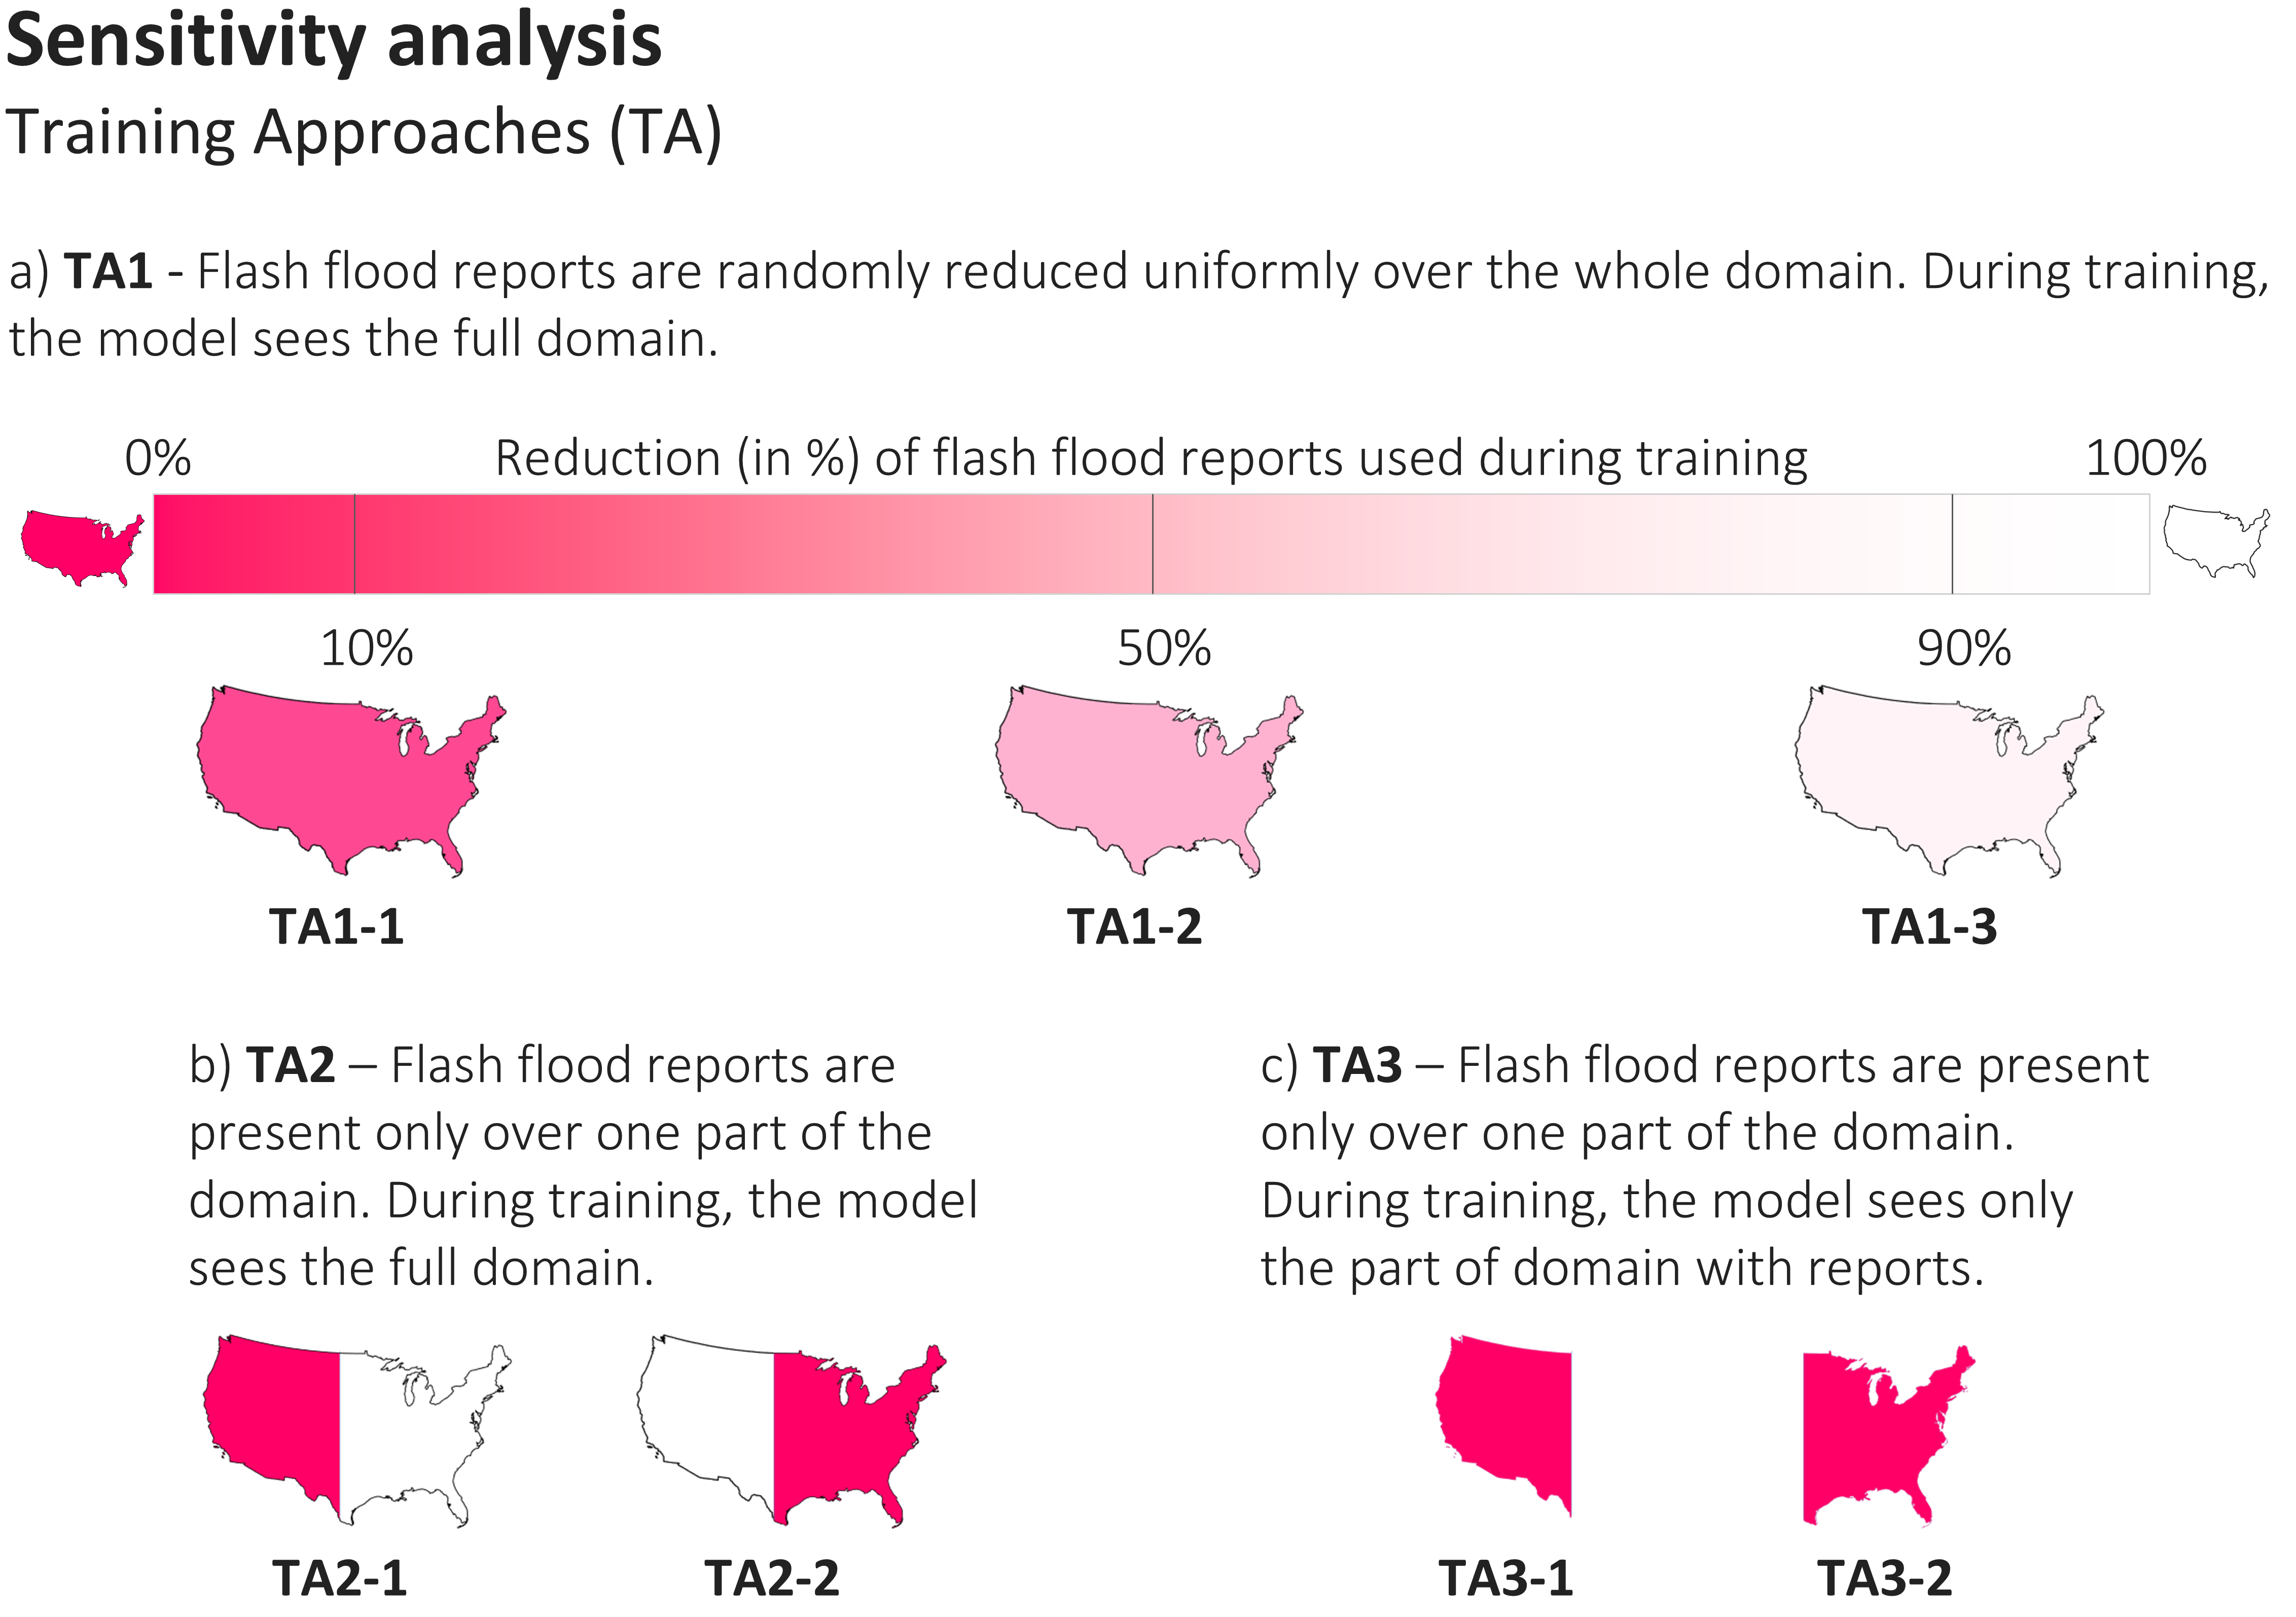
\includegraphics[width=\textwidth]{training_approaches.png}
\caption{\textbf{Training approaches adopted in sensitivity analysis.} Panel (a) describes the Training Approach 1 (TA1) - the randomly reduced-density training dataset. Panel (b) describes Training Approach 2 (TA2) - the sparse regional training dataset. Panel (c) describes the Training Approach 3 (TA3) - the domain-restricted training.}
\label{fig:training_approaches}
\end{figure}

This \marginpara{Training approach 1 (TA1): randomly reduced density} approach tests whether training over the full CONUS domain remains effective when flash flood observations are systematically reduced. Flash flood reports from the Storm Event Database were randomly sampled at three levels: 90\%, 50\%, and 10\% of the original dataset. The sampling was applied uniformly across the entire domain, maintaining the spatial distribution whilst reducing observation density. This approach simulates the scenario of training a global model with sparse but spatially distributed observations.

The \marginpara{Training approach 2 (TA2): sparse regional coverage} second approach maintains training over the full CONUS domain but restricts flash flood observations to specific regions. Unlike Approach 2, the model receives hydro-meteorological data from the entire domain during training but only has access to flash flood labels in the selected region. The non-selected regions contribute only negative samples (non-flood events) to the training dataset. This configuration simulates the realistic scenario of developing a global model where flash flood reports are available only from certain countries or regions, whilst meteorological data has global coverage.

The \marginpara{Training approach 3 (TA3): domain-restricted training} third approach examines whether models trained on high-quality observations from limited geographical regions can effectively predict flash floods in areas where they have never observed any events. The CONUS domain was divided into four regions: East (east of 98°W), West (west of 98°W), North (north of 37°N), and South (south of 37°N). For each configuration, the model was trained using flash flood observations from only one region, with the remaining regions containing no observations during training. The trained model was then applied to predict flash floods across the entire CONUS domain. This approach directly addresses the scenario where certain parts of the world have excellent observational infrastructure, whilst others have none.

The spatial divisions for Approaches 2 (Figure \ref{fig:training_approaches}b) and 3 Figure \ref{fig:training_approaches}c were selected to create regions with varying flash flood characteristics. Two main regions were selected. The eastern region (east of the longitude 100°W) encompasses mostly flat regions (except for the Appalachian Mountains), is highly populated, and is frequently affected by convective storms and hurricanes. The western region (west of the longitude 100°W) encompasses mostly mountainous regions (except for the Central-North Pacific coast), is less populated, and is more frequently affected by large-scale systems bringing large amounts of rainfall due to orographic enhancement.

\subsection{Training data configuration}
For all training approaches, the baseline configuration consists of the full Storm Event Database over the CONUS as presented in Chapter \ref{datasets}. The hydro-meteorological features - including ERA5-ecPoint rainfall, ERA5 antecedent soil moisture, vegetation coverage and topography steepness - also remain consistent with those presented in Chapter \ref{datasets} and already used in Chapter \ref{data_driven_flash_floods_short_medium_range}. The training period remains between 2001 and 2020, as well as the verification period from 2021 to 2024.

\subsection{Model configuration}
The analysis employs the XGBoost model developed in Chapter \ref{data_driven_flash_floods_short_medium_range}. The model's hyperparameters remain consistent with those optimised in Chapter \ref{data_driven_flash_floods_short_medium_range} to ensure that performance differences arise solely from training data modifications (exemplified by TA1-3) rather than model architecture changes. 
 
\subsection{Performance evaluation}

Model performance will first be evaluated by determining how the \textit{distribution of predicted probabilities} changes between the three considered training approaches. Thus, violin plots will be built with the predicted probabilities obtained from training the XGBoost model with TA1-3. As a second model performance assessment, the \textit{flash flood detection capability} for the three different training approaches will be assessed. This will be achieved by computing the different number of grid cells indicating a yes-event between the predictions obtained from one of the TAs and the model trained with the full observational dataset (as computed in Chapter \ref{data_driven_flash_floods_short_medium_range}).

Following the assessments mentioned above, objective verification for the three TAs will be carried out over the full CONUS domain, and the results will be compared to those obtained in Chapter \ref{data_driven_flash_floods_short_medium_range} using the complete training dataset. Such a comparison will determine any potential degradation in predictive performance for any of the three TAs. Hence, the same verification scores adopted in Chapter \ref{data_driven_flash_floods_short_medium_range} will also be considered in this chapter, i.e. ROC curves, precision-recall curves, and reliability diagrams as breakdown scores. Area under the ROC (AUC-ROC) and under the precision-recall curves (AUC-PR), together with the frequency bias (FB) will also be considered as overall scores for discrimination ability (AUC-ROC and AUC-PR) and reliability (FB).
 
The verification assessments will conclude with a case-study-based analysis. This type of \textit{subjective} analysis is preferred to analyse the performance of the global predictions because global impact datasets, such as EM-DAT and DesInventar, do not contain enough observations to compute robust statistics from objective verification (as done over the CONUS). For the US, predictions of areas at risk of flash floods obtained from the three TAs will be presented again for Storm Ida (for more details on the specific event, refer to Chapter \ref{datasets}). In this chapter, however, this US-focused case study will be complemented by case studies from other parts of the world (see Table \ref{} for the complete list of events considered in this chapter).

% For South America, the big flash floods in ..., Brazil on ... will be considered. In Europe, the Valencia, Spain flash floods on the 29th of October will be examined. In Africa, the severe ...., Kenya floods on .... will be examined. In Asia, the extreme flash flooding in China in 2021. In Austrial, the flash floods in ...., will be considered.  


%%%%%%%%%%%%%%%%%
\section{Results}

\subsection{Extension of regional training to global application}

\begin{figure}[htbp]
\centering
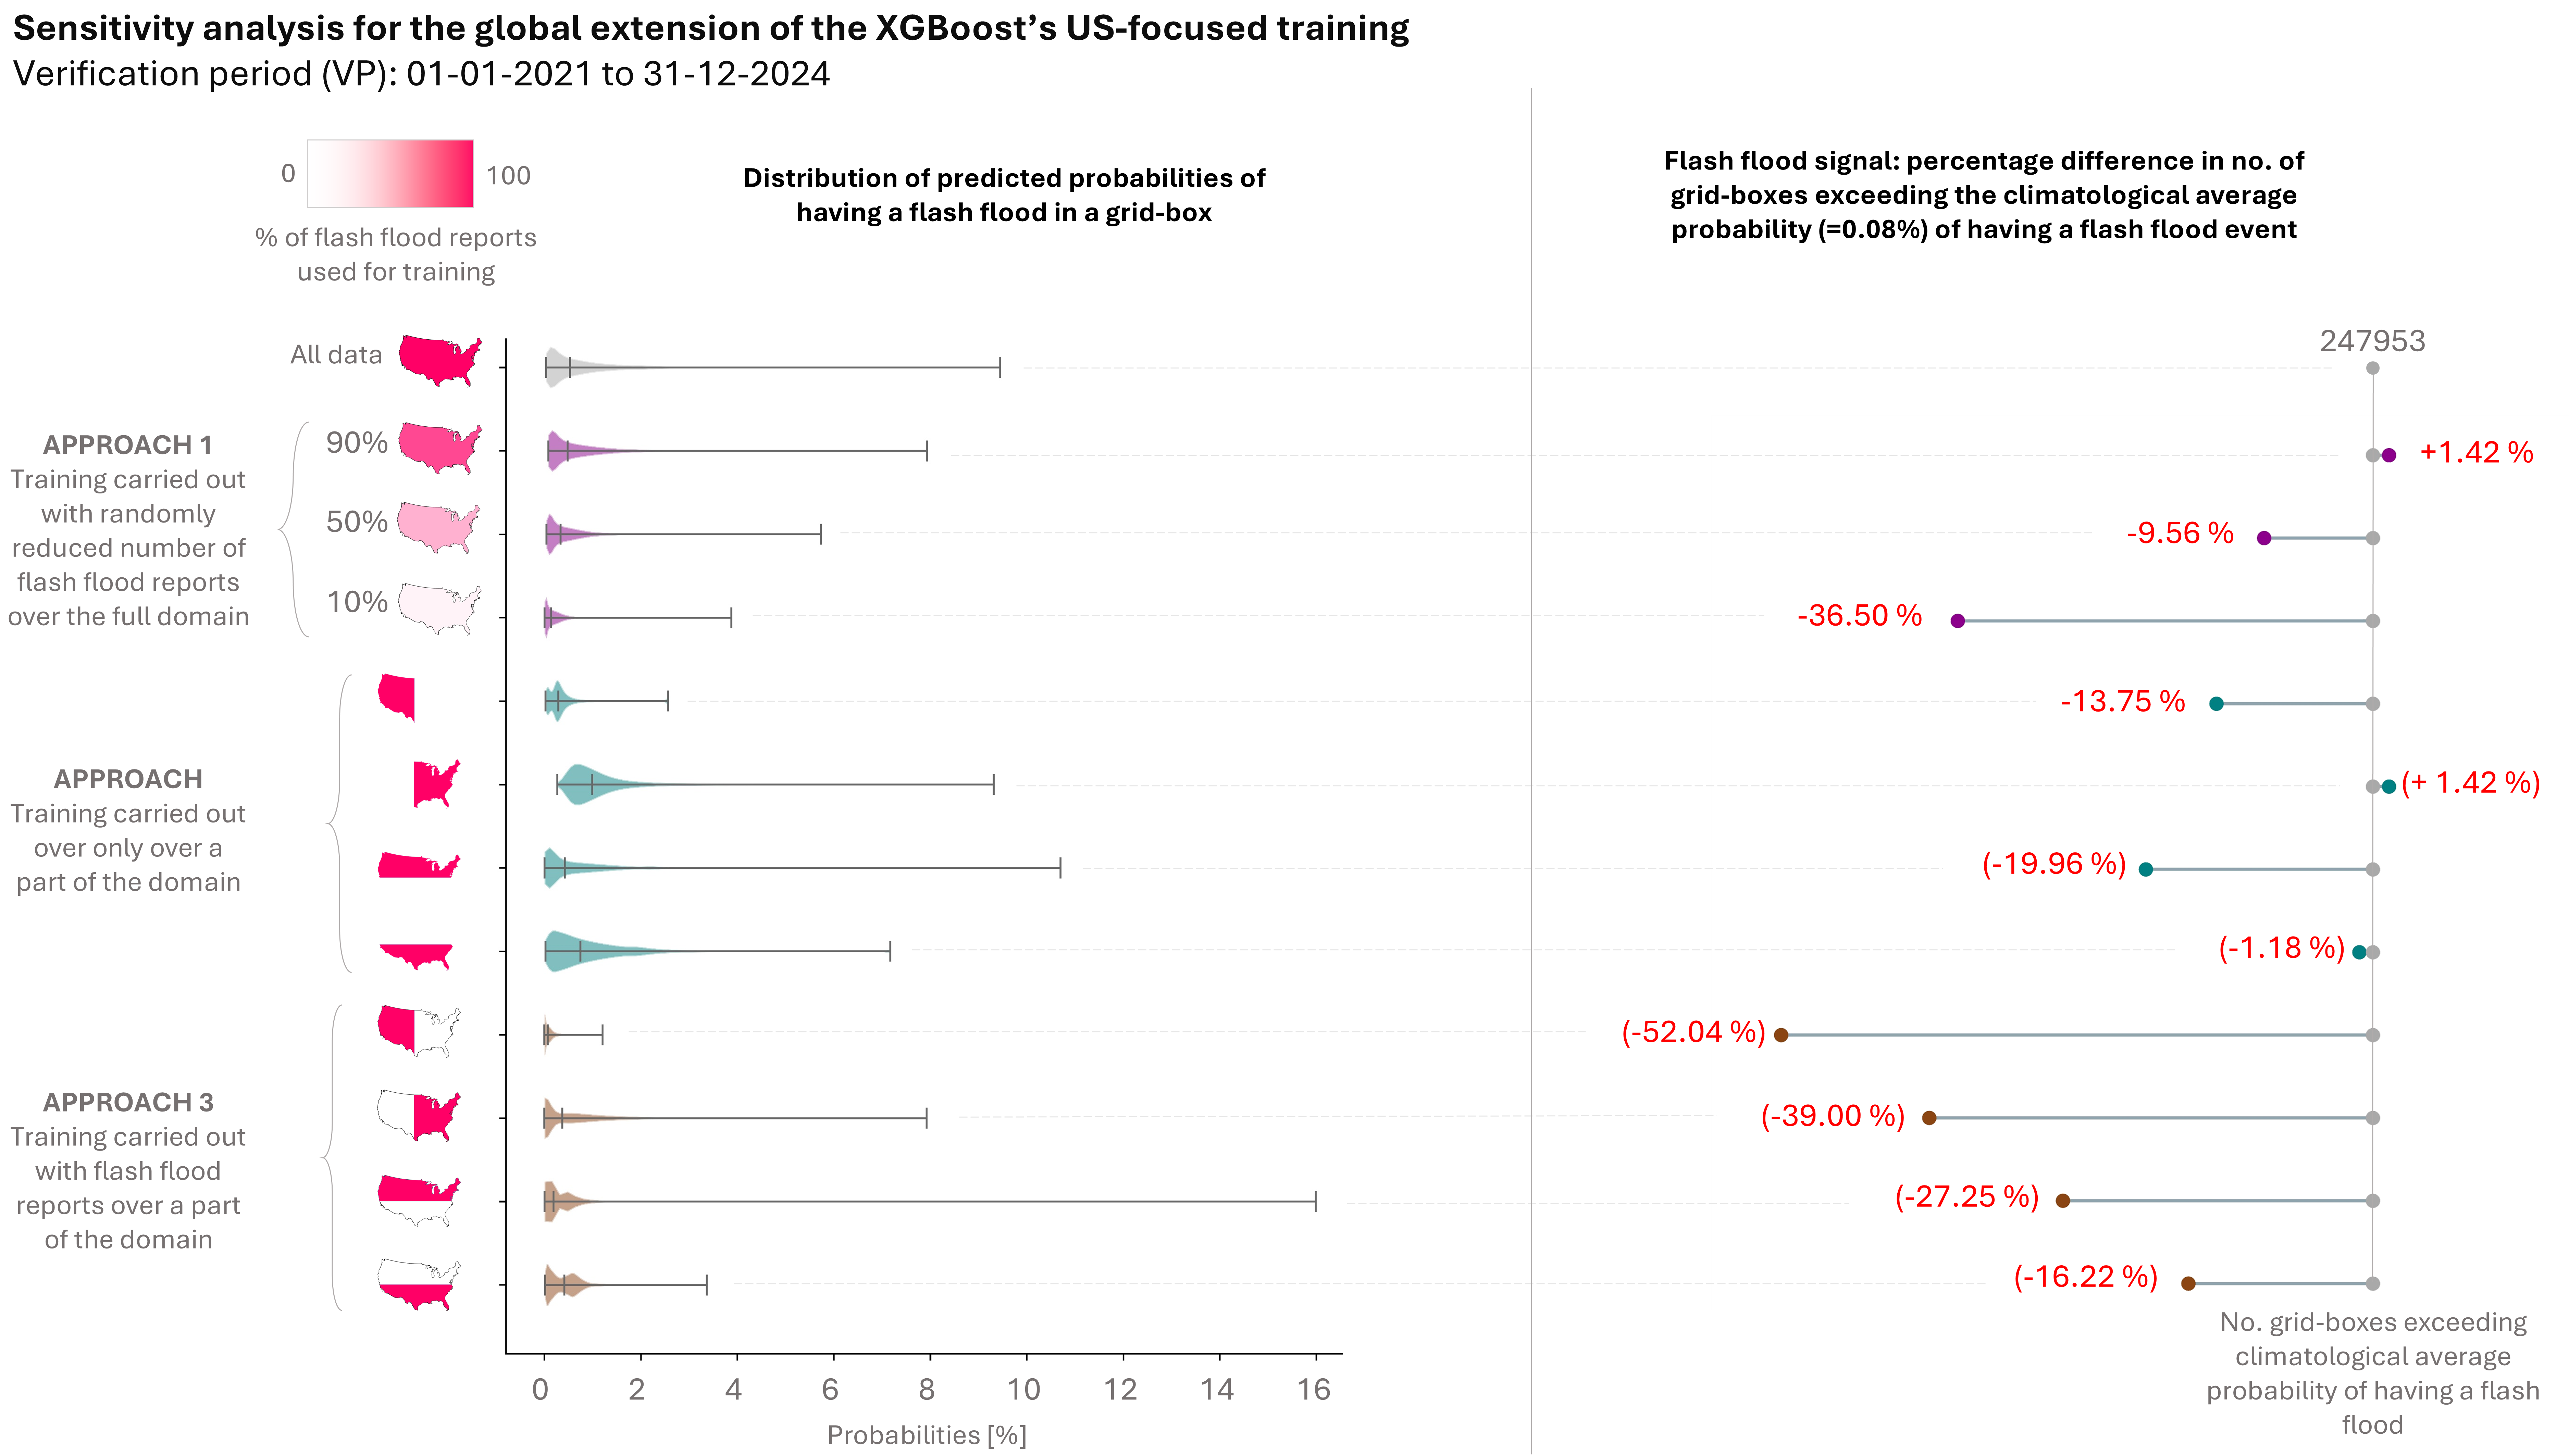
\includegraphics[width=\textwidth]{sensitivity_analysis_global_extension.png}
\caption{\textbf{Global extension performance of regionally-trained XGBoost under different U.S. training data sampling strategies.} Violin plots show predicted probability distributions, whilst dots indicate percentage change in flash flood detection capability relative to climatological baseline. Three approaches tested: random sampling (Approach 1), domain-restricted training (Approach 2), and sub-regional training (Approach 3).}
\label{fig:sensitivity_analysis_global_extension}
\end{figure}

The global application of the regionally-trained XGBoost was evaluated through three distinct approaches, each employing different spatial sampling strategies for training data inclusion (Figure \ref{fig:sensitivity_analysis_global_extension}). The baseline configuration utilising all available flash flood reports in the Storm Event Database, within the verification period, produced a conservative probability distribution, with most predictions remaining below 10\% and 247,953 grid boxes exceeding the climatological average flash flood probability (0.08\%).

Approach 1, which implemented a random reduction of the flash flood reports to predetermined percentages (90\%, 50\%, and 10\%) uniformly, across the entire U.S. domain, demonstrated variable performance. The 90\% sampling configuration merginally increased the detection capability (i.e. number of flash flood reports exceeding the climatological average of flash flood events) by 1.42\%, while the 50\% and the 90\% reductions showed, respectively, a degradation of 9.56\% and 36.50\%, suggesting non-linear relationships between training data volumes and model performance.

Approach 2 explored a spatially-constrained training strategy where the model was trained only over a certain part of the domain where observations are available. The model did not see at all the other part of the domain, and it was applied to create predictions over the whole CONUS domain. This approach simulates a global training that considers only those areas of the world with good observations during training, but uses the model globally to create predictions over the continuous global domain. The reduction in the predicted probabilities was the smallest over the three approaches, with the biggest  reductions of -13.75\% and -19.96\% when the model was trained using the parts of the domain with the smallest number of flash flood reports i.e., the east and the north, respectively. When using the parts of the domain with the biggest number of reports, i.e., the west and the south, there was an increase of +1.42\% and a minimal reduction of -1.18\% of grid-boxes with a flash flood signal.

Approach 3 explores a similar spatially constrained training, where the model is trained over the whole CONUS but with observations only over a restricted part of the domain. This approach simulates a global training of the model over the whole global domain, and considering all available reports. This is the approach with the biggest reduction in predictive ability, with reductions ranging from -52.04\% when the east side was considered and -16.22\% when the south was considered, where training data is most geographically limited.

The varying performance across different training strategies highlights the critical importance of training data representativeness for successful global model deployment. These results show that the distribution of predicted probabilities and the predictive capabilities do change for different data reduction strategies. In all cases, the probability distributions remain highly skewed towards zero probabilities. Such high concentration near the zero value does not surprise as flash floods are rare events. However, the shape and the spread of the probability values varies greatly, with more compressed distributions (with probability values rarely exceeding 2\%) over those cases that train the model with very little training data (cases 4, 5, and 9). Such compression of the probability distribution suggests that the model becomes increasingly conservative and uncertain with less data. When training instead over regions with higher training data volumes (cases 1, 6, 8, 10, and 12), the model seems to be more willing to predict moderate-to-high probabilities. The shape of the distributions is also important. Overall, the shape does not change compared to the baseline (grey violin plot, case 0) with the training approach 1, while the shapes change for approach 2 and 3. The "bulges" in the middle of the distributions, primarily in approach 2, but also in approach 3 suggest the model learned to produce intermediate probabilities (2-6\%), indicating the model developed a more nuanced risk stratification, without losing the capability to predict larger probabilities unless the training dataset is very poor, as in case 5 and 9 represented by the west coast of the CONUS (the area with the least number of flash flood reports over the CONUS). 

The application of these three training strategies suggest that while global applications can maintain reasonable performance under certain conditions, data volumes play a crucial role in determining the transferability of regional flash flood forecasting models to global applications. Due to the presented results, approach 2 is selected for the global application of the CONUS-focused training, i.e., the regional training over the CONUS, using only the Storm Event Database, is applied to global fields to create predictions of areas at risk of flash floods over a continuous global domain. While it is not possible to run a robust verification analysis over the whole global domain due to the sparse density of global datasets like EM-DAT and DesInventar, section \ref{verif_case_study} will provide a selection of case studies over the CONUS and around the world to examine the performance of the regional and global training.


\subsection{Catalogue of flash flood events}
\label{verif_case_study}


%%%%%%%%%%%%%%%%%%%%%
\section{Discussions}


%%%%%%%%%%%%%%%%%%%%%
\section{Conclusions}